% Figure: Grad-CAM, 3 architectures x 5 test images
% Source   : artifact/person1/gradcam/  (repo ManifoldsTeam/WoodID, branch p1,
%            commit d39a3f6b2cc5942e1e718c0dca86e89b0d81eb4d; see SOURCE.txt)
% Checkpoints: seed-42 runs of the same registry used elsewhere in this paper
% Manifest : artifact/person1/gradcam/{gradcam_manifest.csv,
%            sample_selection.csv, gradcam_metadata.json}
%
% NOTE ON ROW LABELS. The row labels printed in the figure follow botanical
% family and therefore show Araucariaceae for Araucaria araucana. This paper
% uses the four-family scheme of docs/references/WoodID_plan.md, in which that
% species is grouped with Pinaceae. The caption below names rows by species to
% avoid the clash; the figure itself should be regenerated with four-family
% labels before submission.
\begin{figure}[!htbp]
\centering
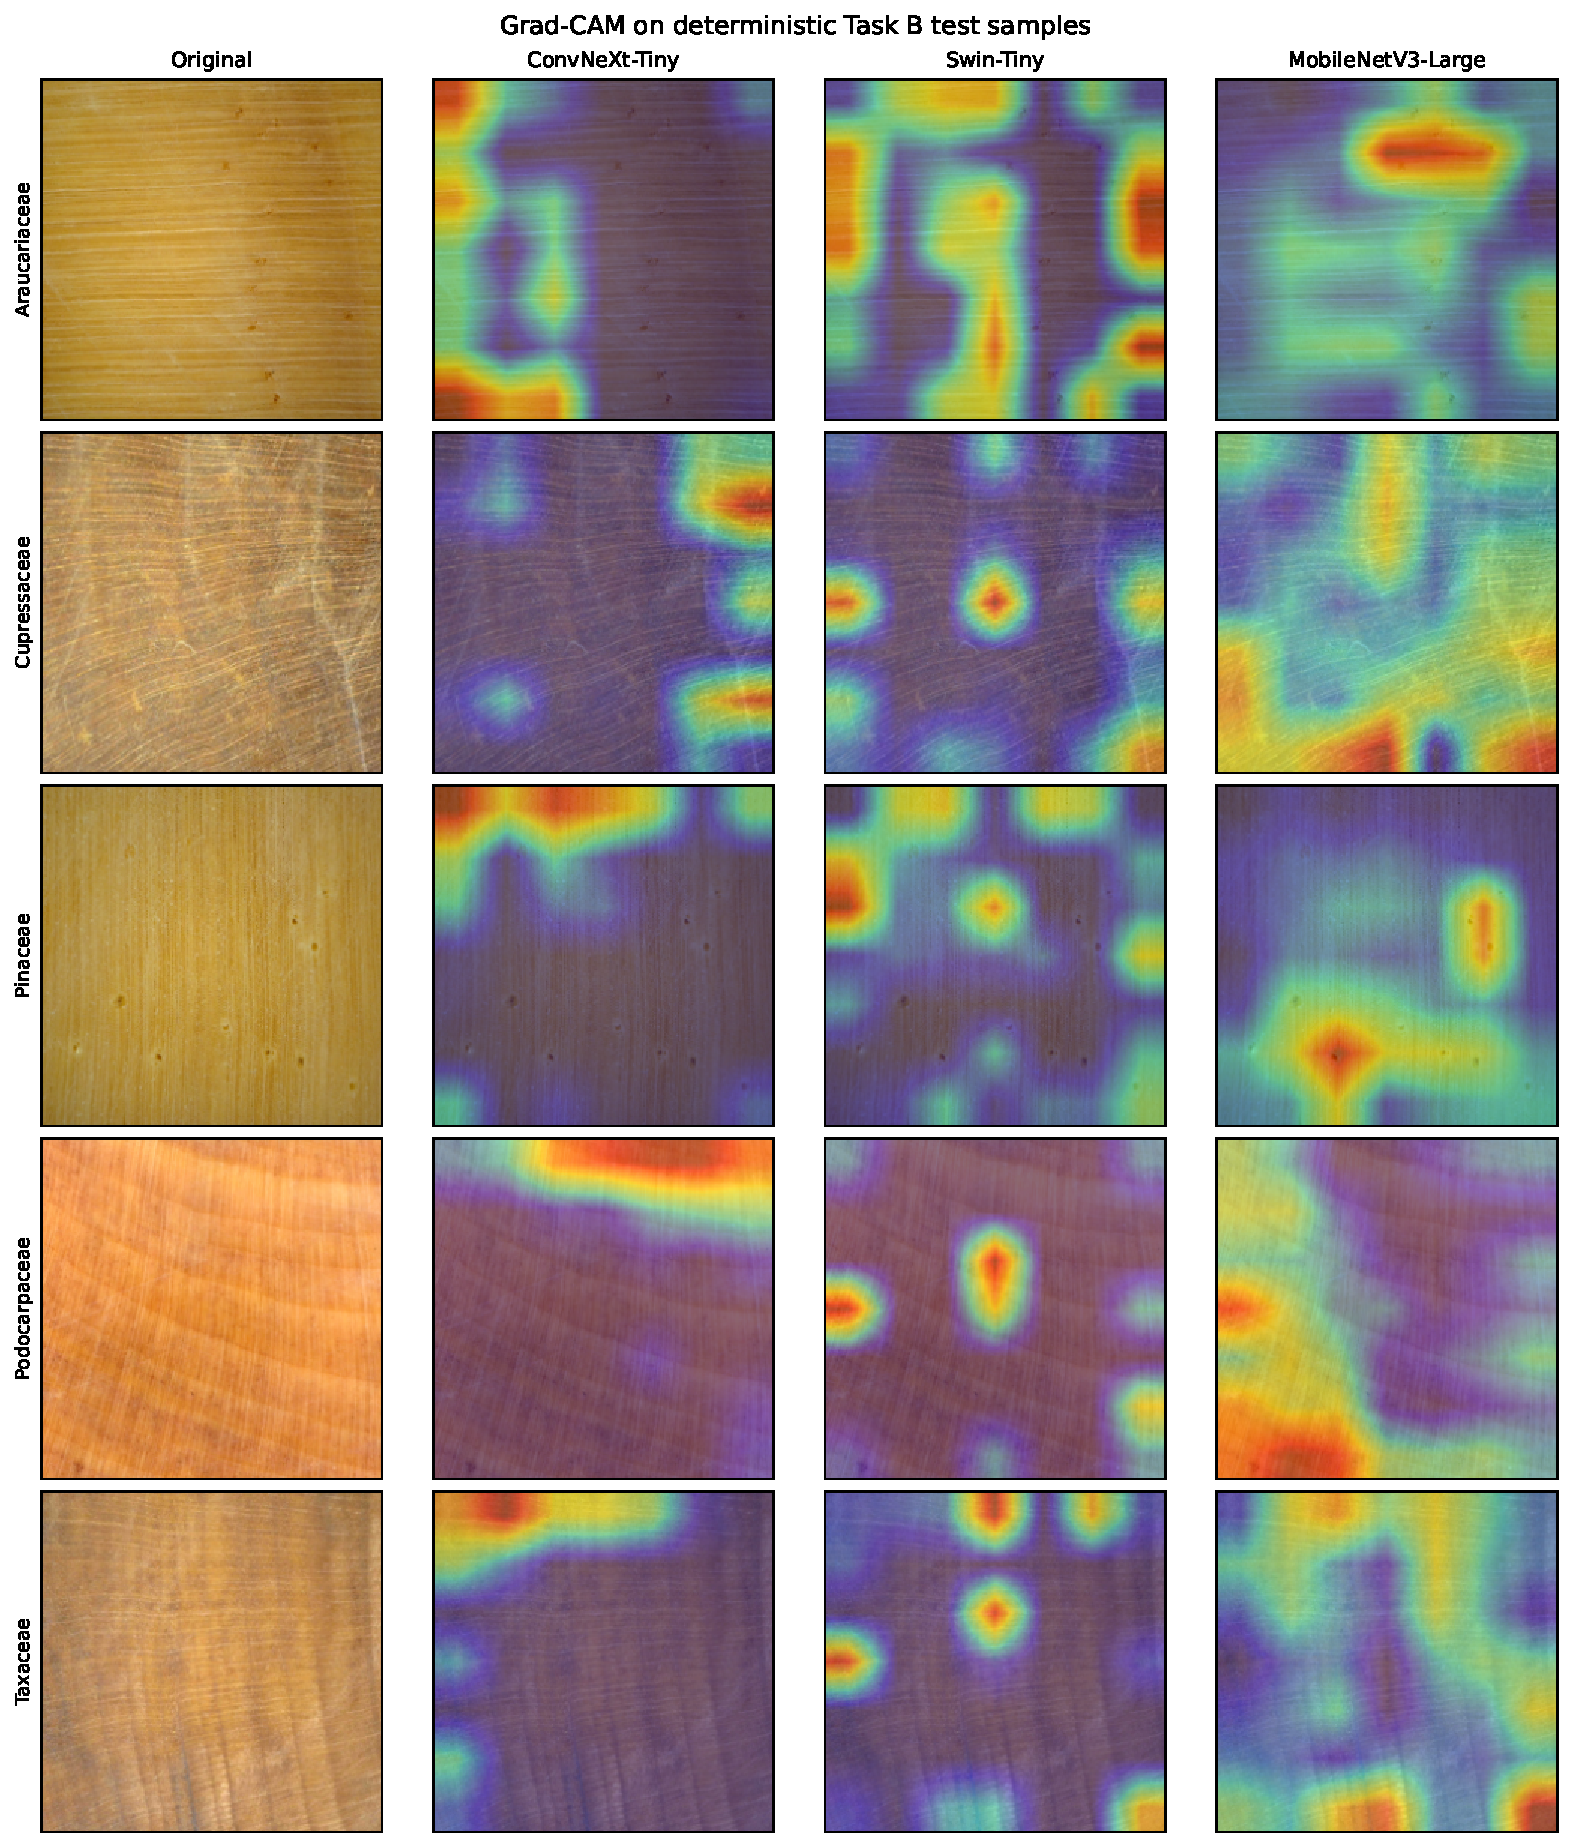
\includegraphics[width=\columnwidth]{artifact/person1/gradcam/fig_gradcam.pdf}
\caption{Bản đồ Grad-CAM cho ConvNeXt-Tiny, Swin-Tiny và MobileNetV3-Large trên năm ảnh test Task~B, mỗi họ một ảnh: \textit{Araucaria araucana}, \textit{Calocedrus rupestris}, \textit{Pinus radiata}, \textit{Podocarpus pilgeri} và \textit{Taxus wallichiana}. Ảnh được chọn theo quy tắc cố định trước: trong số những ảnh cả ba mô hình đều phân loại đúng, lấy ảnh gần nhất với mức độ tin cậy trung vị của ConvNeXt-Tiny trong họ của nó, phá hòa bằng đường dẫn ảnh. Không ảnh nào được chọn vì heatmap trông đẹp. Mỗi bản đồ đều lấy từ checkpoint seed 42 của các lần chạy ở Bảng~\ref{tab:task_b}. Các vùng quy gán trải rộng và ba kiến trúc làm nổi bật những vùng khác nhau trên cùng một ảnh; Grad-CAM định vị nơi gradient tựa vào và tự nó không xác định được đặc trưng nào đang được sử dụng.}
\label{fig:gradcam}
\end{figure}
